% ----------------------------------------------------------------------------------------------------------
% Die Einleitung
% ----------------------------------------------------------------------------------------------------------
\section{Einleitung}\label{einleitung}
Die Möglichkeit eine Oberfläche in ihrer Beschaffenheit 3D zu erfassen, birgt viele Anwendungsfälle. Sei es, um ein 3D-Abbild von einem Raum digital zu erhalten oder in der Industrie Bauteile zu vermessen und auf Fehler zu prüfen. Dabei sind viele verschiedene Verfahren über die Zeit entwickelt und optimiert wurden. 3D Kameras oder auch RGB-D Kameras finden heute vielfältig ihren Einsatz. Diese Arbeit beschäftigt sich mit der Dokumentation und Evaluation eines im Rahmen meiner Praktikumsphase an der Technischen Hochschule Mittelhessen entwickelten Lasertriangulationssensor. Ziel dieser Arbeit ist es dabei, die Funktionalität und Architektur dieses Sensors zu erklären. Zusätzlich soll der Sensor evaluiert und auf bestimme Aspekte mit dem aktuellen Stand der Technik im Bereich der 3D-Kameras bzw. RGB-D Kameras verglichen werden.
Sinn und Zweck eines  \linebreak Lasertriangulationssensor ist es eine Oberfläche zu rekonstruieren und dabei nicht nur die Tiefen-Informationen, sondern auch die Farbinformationen gemeinsam aufzunehmen. Als Verfahren wird, wie im Namen genannt, die Lasertriangulation verwendet.

	\subsection{Aufgabe / Motivation}
	Die grundsätzliche Aufgabe und Motivation entstand durch ein Projekt in Zusammenarbeit mit der Firma RINNTECH – „Technik zur Prüfung von Bäumen“. Die Firma bezeichnet sich selbst wie folgt: „Als Anwender und Entwickler verfügen wir über jahrelange Erfahrung und zahlreiche Patente auf dem Gebiet der Baum- und Holzanalyse. Für diese Anforderungen können wir Ihnen daher ausgereifte Technik und umfassenden Service anbieten“ [Vgl.: RIN]. Beispielanwendungen, für die Geräte und Software bereitgestellt werden sind zum Beispiel Bäume kontrollieren, Jahrringe analysieren, Holzkonstruktionen kontrollieren und Holzqualität und Zuwachs im Wald kontrollieren [Vgl.:  RIN]. Das zugrundeliegende Projekt wurde als Forschungs- und Entwicklungsprojekt zusammen mit dem Institut für Technik und Informatik (ITI) an der THM gestartet. Es trägt den Titel
	
	\textit{"Entwicklung einer Messmethodik zur Ermöglichung einer schnellen Bestimmung von Holzart und -herkunft anhand von Jahrring- und Farbanalyse. Entwicklung der Messwerterfassung und -auswertung der neuen Messmethodik"}
	
	und beschäftigt sich konkret mit der Jahrringanalyse. Durch diese soll Holzart und Herkunft bestimmt werden. RINNTECH verkauft das Produkt „LINTAP“ für diesen Zweck [Vgl.: LINTAP]. Das schon existierende Produkt soll in dem Projekt erweitert, optimiert und automatisiert werden. Die Grundidee besteht darin, dass ein Roboter-Arm mit einer hochauflösenden Kamera über das Objekt fährt und entsprechende Bilder aufnimmt, die für die Jahrringanalyse erforderlich sind. Hier wird eine Kamera eingesetzt, die von dem Roboterarm nah an das Holz herangeführt werden muss. Die Pfade, die der Roboter dementsprechend abfahren muss, müssen also mit hinreichender Genauigkeit errechnet werden. Dazu ist eine digitale Abbildung des Holzes unverzichtbar. Anhand einer rekonstruierten Oberfläche können die entsprechenden Pfade für den Roboter ohne Probleme errechnet werden. Es muss also initial eine Oberflächen-Rekonstruktion des Objektes stattfinden. An diesem Punkt setzt meine Arbeit an. Es wurde eine Software entwickelt, die mithilfe einer Kamera und einen Linienlaser einen 3D-Scan durchführt. Dabei werden die Tiefeninformationen und auch Farbinformationen aufgenommen und verarbeitet. Man erhält eine Punktewolke der gescannten Oberfläche die entsprechend gefärbt ist. Ein typischer Output für eine 3D-Kamera in der Industrie. Die  \linebreak Aufgabenstellung wurde noch etwas konkretisiert. Als Methode soll eine Lasertriangulation verwendet werden, dazu wurde die Kamer und der Linienlaser bereitgestellt. Zusätzlich soll nur Open-Source-Software verwendet werden und die Anwendung soll über ROS2 (Robot Operating System) laufen.
	
	\subsection{Stand der Technik}
		\subsubsection{Methodik}
		Lasertriangulation ist nicht die einzige Methode eine Oberflächen-Rekonstruktion  \linebreak durchzuführen. Die zentralen Technologien zu diesem Zweck sind Triangulation oder Time-of-Flight [Vgl.: SotA]. 
		Bei der Triangulation gibt es zwei Ansätze. Einen direkten über Structured Light. Dabei wird ein bekanntes Muster mit einem Laser oder Ähnlichem auf die Oberfläche projiziert. Eine Kamera nimmt das Muster als Bild auf, welches sich durch die variierende Höhe und Form der Oberfläche verzerrt. Diese Verzerrung wird als Anhaltspunkt verwendet, um die Unterschiedlichkeiten in der Höhe zu ermitteln. Lasertriangulation und der hier verwendete Lösungsansatz gehören zu dieser Möglichkeit. 
		Einen indirekten Ansatz der Triangulation bietet Stereo-Vision. Dabei werden zwei Kameras verwendet, die zwei aufgenommenen Bildern aus unterschiedlichen Positionen liefern. Ebenfalls wird ein fester Punkt benötigt, der auch mit einem Laser oder Ähnlichem im Bild projiziert werden kann. Über die zwei unterschiedlichen Bilder kann die Position ermittelt werden.
		
		Die Time-of-Flight-Technologie benutzt eine andere Lösungsmöglichkeit. Es wird Licht auf einen Punkt auf der Oberfläche gestrahlt. Dort wird es zurück reflektiert und von einem Sensor registriert. Dieser misst die verstrichene Zeit. Durch die bekannte  \linebreak Geschwindigkeit von Licht, kann über die gebrauchte Zeit der zurückgelegte Weg errechnet werden. Dieser entspricht der Höhe.
	
		\subsubsection{Geräte}
		Diese Methoden finden ihre Anwendung auch in der Industrie. Diverse Geräte und Anwendungen zur Oberflächen-Rekonstruktion sind bereits auf dem Markt. Die Rede ist von sogenannten 3D-Kameras bzw. RGB-D Kameras. Dabei steht RGB (Red, Green, Blue) für die Farbinformationen und das D (Depth) für die Tiefeninformation. Angefangen mit der von Microsoft entwickelten „Kinect“ über die „Intel RealSense“ zur „Google Tango“ folgen viele weitere Geräte. Diese sind nicht nur meist für einen geringen Preis verfügbar, sie könne auch die entsprechenden Pixelfarben in einer guten Auflösung  \linebreak aufnehmen.
		Zusätzlich geschieht die Aufnahme in Echtzeit, was bedeutet, dass sich die herausgegebene Punktewolke ändert, sobald sich die aufgenommene Oberfläche ändert bzw. die Kamera bewegt wird.
			
	\subsection{Kriterien}
	Für das Projekt wurde zu Beginn eine „Intel RealSense d415“ verwendet. Die Industrie-3D-Kamera erfüllt die Anforderungen. Es kann eine 3D-Rekonstruktion des Objektes mit Farbinformationen durchgeführt werden. Die RealSense verwendet Stereo-Vision-Technologie. Sie verfügt über zwei Kameras und einen Projektor für ein vom Menschen nicht sichtbares Infrarot-Muster. Die Kamera berechnet so für jeden Pixel seine 3D-Position in Echtzeit. In dem Forschungsprojekt wurde jedoch auch überlegt, ob man die 3D-Rekonstruktion jenseits eine Industrie-Lösung erhalten kann. Grundsätzlich ist dafür eine einfache Webcam mit einem Linienlaser ausreichend. So kam die Idee einen Open-Source Lasertriangulationssensor zu entwickeln.
	Dieser soll mit der Intel RealSense und dem generellen Industriestandart von RGB-D Kameras verglichen werden. Dabei ist die Genauigkeit (der Tiefeninformationen), Schnelligkeit des Scans und die Auflösung der Farbinformationen ausschlaggebend. Sowohl die Intel RealSense als auch die Open-Source-Variante sollen am Ende eine Punktewolke liefern. Diese kann direkt verglichen werden. Genauso können die Position der Punkte auf eine Genauigkeit untersucht werden. 
	
	\subsection{Lösungsansatz}
	Um den genaueren Erklärungen im Hauptteil folgen zu können, soll einmal oberflächlich der Lösungsansatz der entwickelten Anwendung erläutert werden. Die Grundlegende Idee ist die Lasertriangulation. Dafür ist eine Kamera und ein Projektor für eine Laserlinie notwendig.
	
	\begin{figure}[h]
		\centering
		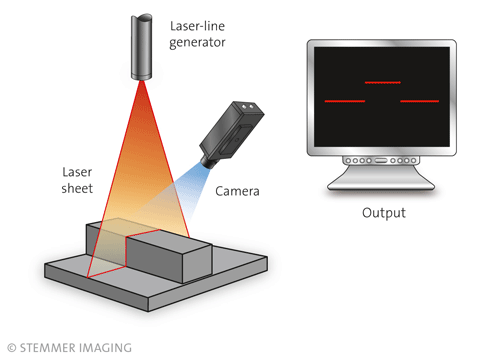
\includegraphics[height=7cm]{img/grundlagen/lasertriangulation_1}
		\caption{Lasertriangulation}
		\label{lasertriangulation}
	\end{figure}
	
	Die resultierende Punktewolke der 3D-Rekonstruktion muss im Bezug zu einem Koordinatensystem stehen. Als Bezugspunkt wird die Kamera gewählt. Das bedeutet, dass sich die Koordinaten auf die Kamera beziehen und sich der Ursprung des Koordinatensystems an den optischen Sensor der Kamera befindet. Für die Berechnung von einem Pixel zu einem 3D-Punkt wird die Ebene bestimmt, die der Laser projiziert. Ausgehend von dem Startpunkt des Projektors und der projizierten Linie kann das Laserlicht als Ebene begriffen werden. Diese Ebene kann aus Kamerasicht als Ebenengleichung berechnet werden. In der Theorie wird dann, sobald die Ebenengleichung bekannt ist, eine Laserlinie auf die zu scannende Oberfläche projiziert. Die Kamera nimmt ein Bild von dieser Oberfläche auf. Über Bildverarbeitung wird aus dem aufgenommenen Bild die rote Laserlinie herausgearbeitet. In Abb. 1 wird unter Output Beispielhaft das Ergebnis dieses Prozesses gezeigt. Die Pixel der Laserlinie werden im nächsten Schritt auf die Ebene gespannt, indem sie in die Ebenengleichung eingesetzt werden. Dadurch wird eine dritte Dimension für die Pixel errechnet. Die 3D-Punkte sind dann, wie gefordert, aus Sicht der Kamera. Diese Methodik liefert die 3D-Represäntation der Laserlinie, jedoch nicht von dem kompletten Objekt. Der Sensor (bestehend aus der Kamera, den Laser und der Software zusammen) muss zusätzlich über das Objekt bewegt werden. Die Aufgenommenen Linien werden dann zu einer gesamten Punktewolke zusammengefügt. Dabei muss bekannt sein, welche Strecke an Bewegung von dem Sensor zurückgelegt wurde, um die neue Linie in der richtigen Position einzufügen. 
